%=========================================
% 	   Sicherheit						 =
%=========================================
\section{Sicherheitsaspekte}

Jede Anwendung muss eine sichere Umgebung zur Verfügung stellen. Vor allem 
Webanwendungen bedürfen oft besonderer Sicherheit, da schlechtere Javascript-
Implementierungen mit einigen Tricks umgangen werden können und Nutzer dadurch 
Zugriff auf Daten erhalten können, welche nicht für sie bestimmt sind. Einige 
Fragen müssen durchdacht werden, um eine nachhaltige Implementierung der 
Sicherheitsmechanismen zu gewährleisten:

\begin{itemize}
\item Wie werden Authentifizierung und Authorisierung sichergestellt?
\item Müssen beim Austausch des / der Server die Sicherheitsmechanismen neu implementiert und / oder die
	  Sicherheitseinstellungen neu konfiguriert werden?
\item An welchen Stellen der Anwendung werden sensible Daten übertragen und bedürfen kryptografischer 	      
      Verschlüsselung?
\end{itemize} 

Dieser Abschnitt zeigt, wie wir das Spring Framework nutzen, um eine sichere 
Umgebung und damit auch alle damit in Verbindung stehenden Sicherheitsanliegen 
gewährleisten.

\subsection{Spring Security Module}
\label{subsec:spring_security}

Das Spring Framework stellt den Service Spring Security zur Verfügung, welcher grundsätzlich genutzt 
werden kann, um alle oben genannten Problemstellungen zu lösen. Insgesamt stellt Spring Security folgende 
elf Module zur Implementierung von Sicherheitsmechanismen bereit:

\begin{table}[hbt]
 \caption{Spring Security Module}
  \begin{tabular}{lp{11cm}}
    \toprule 
    \textbf{Module} & \textbf{Description} \\
    \hline
    ACL & Provides support for domain object security through access control lists (ACLs) \\
    %------------------------------------------------------------------------------------------
    Aspects & A small module providing support for AspectJ-based aspects instead of standard
	Spring AOP when using Spring Security annotations. \\
	%------------------------------------------------------------------------------------------
	CAS Client Support & for single sign-on authentication using Jasig’s Central Authentication
	Service (CAS). \\
	%------------------------------------------------------------------------------------------
	Configuration & Contains support for configuring Spring Security with XML and Java. 
	(Java configuration support introduced in Spring Security 3.2.) \\
	%------------------------------------------------------------------------------------------
	Core & Provides the essential Spring Security library. \\
	%------------------------------------------------------------------------------------------
	Cryptography & Provides support for encryption and password encoding. \\
	%------------------------------------------------------------------------------------------
	LDAP & Provides support for LDAP-based authentication. \\
	%------------------------------------------------------------------------------------------
	OpenID & Contains support for centralized authentication with OpenID. \\
	%------------------------------------------------------------------------------------------
	Remoting & Provides integration with Spring Remoting. \\
	%------------------------------------------------------------------------------------------
	Tag Library & Spring Security’s JSP tag library. \\
	%------------------------------------------------------------------------------------------
	Web & Provides Spring Security’s filter-based web security support. \\
	\bottomrule
  \end{tabular}
\end{table}

Normalerweise werden nicht alle Module benötigt. Auch bei uns werden nur die Module Core, 
Configuration und Web eingesetzt. Der in einem vorherigen Kapitel vorgestellte Service Maven wird an 
dieser Stelle eingesetzt, um sämtliche benötigte Module, welche als .jar Dateien geliefert werden, zu 
importieren.

\subsection{Implementierung und Funktionsweise}

Um Spring Security aktiv in der Anwendung nutzen zu können muss als erstes eine springSecurityFilterChain 
Klasse implementiert werden. Wie der Name der Klasse schon sagt, handelt es sich dabei um einen Filter, der 
jegliche ankommende Webanfragen durch alle implementierten Sicherheitsmechanismen laufen lässt, sozusagen 
verkettet, und den Einsatz von Spring Security so erst ermöglicht. Das folgende Diagramm stellt den 
grudsätzlichen Ablauf einer Anfrage und deren Filterung durch Sicherheitsmechanismen dar.

\begin{figure}
    \centering
    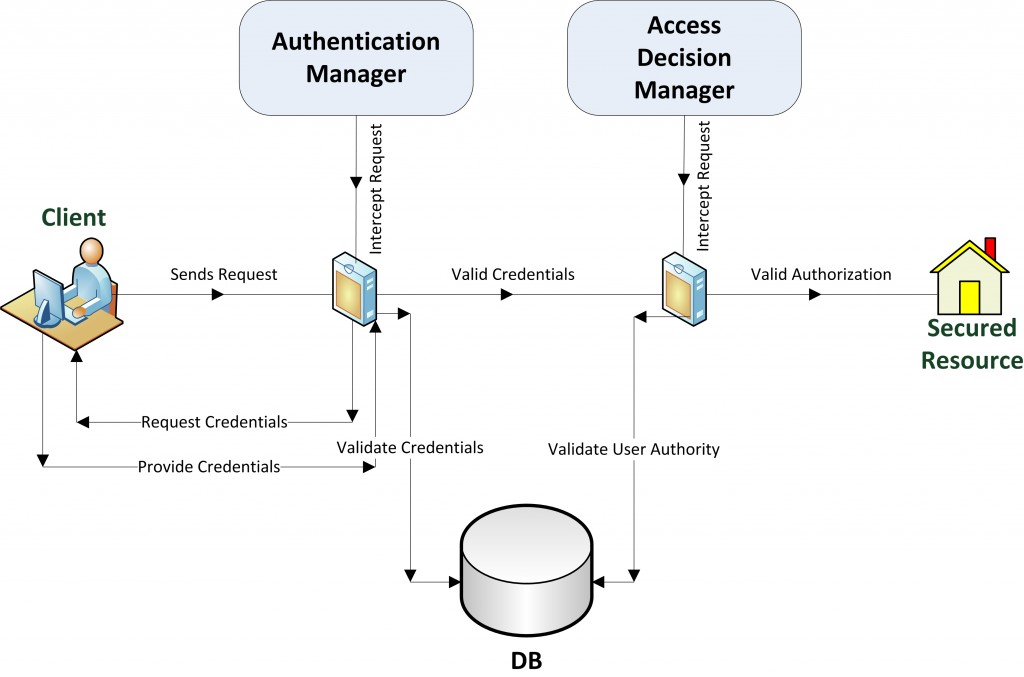
\includegraphics[width=0.85\textwidth]{Graphics/security/user_privileges}
    \caption{Authentifizierung und Validierung der Privilegien eines Nutzers}
   \label{fig:user_privileges}
\end{figure}

Stellt ein Client nun eine Anfrage an eine Ressource, wird diese erst durch einen implementierten 
Authentication-Manager gefiltert. Die verschiedenen Unterfilter werden durch Authentication-Provider 
realisiert. Der Authentication-Provider prüft die beim Login eingegebenen Daten auf ihre Richtigkeit. 
Sind die Daten nicht im Code verankert und in einer Datenbank gespeichert, wird hier zusätzlich ein 
Jdbc-user-service benötigt, welcher die nötigen SQL-Anfragen zum Abgleichen der Nutzerdaten als 
Parameter erwartet. Hat der Abgleich mit der Datenbank stattgefunden und die Daten waren korrekt, wird 
die Anfrage weitergeleitet. Im obigen Diagramm wird der folgende Prozess durch den Access Decision 
Manager dargestellt. Dieser ist in unserer konkreten Anwendung nicht implementiert, jedoch findet der 
Authorisierungsprozess hier trotzdem statt. An dieser Stelle muss überprüft werden, ob der Nutzer die 
nötigen Privilegien besitzt, um eine gewisse Seite aufrufen zu dürfen. Dieser Abgleich wird ebenfalls 
mit in der Datenbank gespeicherten Daten durchgeführt. An dieser Stelle gibt es folgende verschiedene 
Privilegien, die Spring Security zur Authorisierung zur Verfügung stellt: \newpage

\begin{table}[hbt]
 \caption{Die verschiedenen von Spring zur Verfügung gestellten Privilegien}
  \begin{tabular}{lp{9.5cm}}
    \toprule 
    \textbf{Expression} & \textbf{Description} \\
    \hline
    \texttt{hasRole([role])} & Returns \texttt{true} if the current principal has the specified role \\
    %------------------------------------------------------------------------------------------
    \texttt{hasAnyRole([role1,role2])} & Returns \texttt{true} if the current principal has any of the supplied roles (given as a comma-separated list of strings) \\
	%------------------------------------------------------------------------------------------
	\texttt{principal} & Allows direct access to the principal object representing the current user \\
	%------------------------------------------------------------------------------------------
	\texttt{authentication} & 	Allows direct access to the current \texttt{Authentication} object obtained from the \texttt{SecurityContext} \\
	%------------------------------------------------------------------------------------------
	\texttt{permitAll} & Always evaluates to \texttt{true} \\
	%------------------------------------------------------------------------------------------
	\texttt{denyAll} & Always evaluates to \texttt{false} \\
	%------------------------------------------------------------------------------------------
	\texttt{isAnonymous()} & Returns \texttt{true} if the current principal is an anonymous user \\
	%------------------------------------------------------------------------------------------
	\texttt{isRememberMe()} & Returns \texttt{true} if the current principal is a remember-me user \\
	%------------------------------------------------------------------------------------------
	\texttt{isAuthenticated()} & Returns \texttt{true} if the user is not anonymous \\
	%------------------------------------------------------------------------------------------
	\texttt{isFullyAuthenticated()} & Returns \texttt{true} if the user is not an anonymous or a remember-me user \\
	\bottomrule
  \end{tabular}
\end{table} 
\bigskip
Wird auch dieser Abgleich erfolgreich durchgeführt, erhält der Nutzer Zugriff auf die Ressource. Das 
folgende Codesegment veranschaulicht unsere Implementierung, dieser Sicherheitsmechanismen: \\

\lstinputlisting [style=XML]{Snippets/security.xml}

Das durch den Authentication-manager gekennzeichnete Codesegment zeigt die Implementierung des 
Validierungsprozesses der Logindaten.
Anhand des zweiten Abschnitts des Codesegments lässt sich erkennen, dass in unserer Anwendung z.B. die 
Startseite und die Seite zum Erstellen eines neuen Accounts von jedem Nutzer aufgerufen werden darf, 
da das access Attribut hier auf \texttt{permitAll} gesetzt wurde. Das Anzeigen der Tweets benötigt 
jedoch erst eine Authentifizierung, da der access Parameter den Wert \texttt{isAuthenticated()} 
annimmt. Natürlich könnten hier auch spezielle Bereiche für Administratoren eingerichtet werden. Das 
access Attribut müsste dort lediglich dementsprechend parametrisiert  und die Authorität in der 
Datenbank hinterlegt werden.

\subsection{Verschlüsselung sensibler Daten}

Die vorherigen Abschnitte haben gezeigt, dass Spring-Security in jeder Situation eine Lösung für die 
geforderte Problemstellung liefert. Auch im Bezug auf das Verschlüsseln von sensiblen Daten wie 
Passwörtern stellt das Modul eine einfache Lösung bereit. Da in unserer Anwendung das Anlegen von 
Accounts möglich sein soll und Passwörter aus Sicherheitsgründen nicht im Volltext in der Datenbank 
abgelegt werden dürfen, wird hier eine angemessene Verschlüsselungsmethode benötigt. Diese 
Verschlüsselung wird durch eine von Spring bereitgestellte passwordEncoder Klasse realisiert. Diese 
ist in der Lage, die eingegebenen Passwörter mithilfe folgender Algorithmen zu verschlüsseln:

\begin{enumerate}
  \item \textit{Bcrypt}: Eine auf dem Blowfish-Algorithmus basierende Funktion
  \item \textit{SHA}: Ein Verschlüsselungsalgorithmus der SHA-1 Familie
  \item \textit{SHA-256}: Ein Verschlüsselungsalgorithmus der SHA-2 Familie
  \item \textit{Md4}: Eine auf 32-Bit Systemen effektive Hashfunktion welche in 128-Bit verschlüsselt
  \item \textit{Md5}: Eine nicht mehr als sicher geltende Hashfunktion, die ebenfalls einen 128-Bit- 	Hashwert erzeugt
\end{enumerate}

Wir haben uns an dieser Stelle für die Verschlüsselung der Passwörter mittels der SHA-256 Hashfunktion 
entschieden, da diese, im Gegensatz zu den meisten anderen oben genannten Funktionen, einen 256-Bit-
Hashwert erzeugt, immer noch als stabil gilt und wir im Laufe des Studiums bisher nur mit den SHA-
Hashfunktionen in Kontakt gekommen sind. \\
Das Einbinden der \texttt{passwordEncoder} Klasse findet ebenfalls im Authentication-manager Abschnitt statt 
und erfordert nur wenige Zeilen: \\

\lstinputlisting [style=XML]{Snippets/security_auth_provider.xml} \newpage

Hierzu wird ein weiterer Authentication-Provider Abschnitt erzeugt, in dem sowohl die Datenbank als 
auch der passwordEncoder und die Art des Hashes als Parameter übergeben werden. Des weiteren muss die 
Klasse selbst eingebunden werden: \\

\lstinputlisting [style=XML]{Snippets/security_password_encoder.xml}
\bigskip 
Die von einem Nutzer eingegebenen Passwörter werden dann mittels SHA-256 verschlüsselt und in der 
Datenbank hinterlegt. \\
Abschließend bleibt zu sagen, dass die meisten von uns genutzten Klassen und in diesem Kapitel 
erläuterten Methoden nur eine Option darstellen, um jeweilige Problemstellungen zu lösen. Spring-
Security ist ein mächtiger Service, der für jede Situation und Umgebung die nötigen Vorraussetzungen 
liefert, sichere und serverunabhängige Anwendungen zu schreiben. Des weiteren müssen von Spring-
Security bereitgestellte Klassen nicht zwangsläufig verwendet werden. Zum Beispiel wäre es möglich, 
einen eigenen Filter zu implementieren und dabei auf die springSecurityFilterChain Klasse zu 
verzichten.









